% This is LLNCS.DEM the demonstration file of
% the LaTeX macro package from Springer-Verlag
% for Lecture Notes in Computer Science,
% version 2.4 for LaTeX2e as of 16. April 2010
%
\documentclass{llncs}
%
\usepackage{makeidx}  % allows for indexgeneration
%

\usepackage{graphicx}
\usepackage[htt]{hyphenat} % for hypenantion of texttt
\usepackage{mathpartir} % for typing rules

% use Times font to save some space
\usepackage{mathptmx}

\usepackage{datetime} % for the date in the draft versions

% \usepackage[T1]{fontenc}
% \newcommand{\changefont}[3]{\fontfamily{#1}\fontseries{#2}\fontshape{#3}\selectfont}
% \newcommand{\ic}[1]{\changefont{cmtt}{m}{n}{#1}\normalfont} %keyword font
\newcommand{\ic}[1]{\emph{#1}} %workaround - the above commands seem to make the
%fonts look different (bad) on some machines

\newcommand{\mv}[1]{\footnote{mv: #1}}
\newcommand{\todo}[1]{\footnote{\textbf{TODO}: #1}}
\newcommand{\ds}[1]{\footnote{ds: #1}}


\usepackage{listings} % http://en.wikibooks.org/wiki/LaTeX/Packages/Listings
\usepackage{multicol}

\usepackage{color}
\definecolor{dkgreen}{rgb}{0,0.6,0}
\definecolor{gray}{rgb}{0.5,0.5,0.5}
\definecolor{mauve}{rgb}{0.58,0,0.82}
\lstset{ %
  language=Java,                % the language of the code
  literate={~} {$\sim$}{1},
  basicstyle=\scriptsize,           % the size of the fonts that are used for
  % the code
  %numbers=left,                   % where to put the line-numbers
  %numberstyle=\tiny\color{gray},  % the style that is used for the line-numbers
  %stepnumber=2,                   % the step between two line-numbers. If it's
  % 1, each line
                                  % will be numbered
  %numbersep=5pt,                  % how far the line-numbers are from the code
  %backgroundcolor=\color{white},      % choose the background color. You must
  % add \usepackage{color}
  showspaces=false,               % show spaces adding particular underscores
  showstringspaces=false,         % underline spaces within strings
  showtabs=false,                 % show tabs within strings adding particular underscores
  %frame=single,                   % adds a frame around the code
  numberbychapter=false,
  belowskip=-15pt,
  %rulecolor=\color{black},        % if not set, the frame-color may be changed
  % on line-breaks within not-black text (e.g. commens (green here))
  tabsize=2,                      % sets default tabsize to 2 spaces
  captionpos=b,                   % sets the caption-position to bottom
  breaklines=true,                % sets automatic line breaking
  breakatwhitespace=false,        % sets if automatic breaks should only happen at whitespace
  columns=fullflexible,
  title=\lstname,                   % show the filename of files included with \lstinputlisting;
                                  % also try caption instead of title
  %keywordstyle=\color{blue},          % keyword style
  %commentstyle=\color{dkgreen},       % comment style
  %stringstyle=\color{mauve},         
  stringstyle=\ttfamily,         % string literal style
  escapeinside={\%*}{*)}%,            % if you want to add a comment within your code
  %morekeywords={*,...}               % if you want to add more keywords to the set
}

\usepackage{float}
%\floatstyle{boxed}
\floatstyle{plaintop}

\newfloat{listing}{tbp}{lol}
\floatname{listing}{Listing}

% \makeatletter
% \let\c@listing\c@lstlisting
% \makeatother

\usepackage{verbatim}
\newenvironment{code} 
    {\vspace{3mm}
     \noindent
     \rule{\textwidth}{0.7pt}
     \vspace{-4mm}
     \scriptsize \verbatim}
    {\endverbatim \normalsize
	 \vspace{-4mm}
	 \rule{\textwidth}{0.7pt}
	 \vspace{0mm}
	 }

\setlength{\floatsep}{.5em}
\setlength{\textfloatsep}{.5em}

\newcommand{\g}{\ensuremath{\Gamma}}
\newcommand{\f}{\ensuremath{\vdash}}
\newcommand{\T}{\mytt{T}}

\newcommand{\mytt}[1]{\textup{\texttt{#1}}}
\newcommand{\mykeyb}[1]{\textup{\textbf{#1}}}

\newcommand{\checkm}{\mytt{@Check}}

\newcommand{\failedexc}{\mytt{RuleFailedException}}
\newcommand{\ruleapptrace}{\mytt{RuleApplicationTrace}}

\begin{document}

%
\pagestyle{headings}  % switches on printing of running heads


\title{Approaches and Tools for Implementing Type Systems in Xtext}

%
%\titlerunning{Xtext Type Systems}  % abbreviated title (for running head)
%                                     also used for the TOC unless
%                                     \toctitle is used
%
\author{Lorenzo Bettini\inst{1} \and Serano
Colameo\inst{2} \and Dietmar
Stoll\inst{2}  \and Markus V\"olter\inst{3}}
%
\authorrunning{Terfloth et al.} % abbreviated author list (for running head)
%
%%%% list of authors for the TOC (use if author list has to be modified)
\institute{Dipartimento di Informatica, Universit\`a di Torino
\and
Itemis Schweiz GmbH
\and
independent/Itemis AG}


\maketitle              % typeset the title of the contribution

\begin{abstract}
\input{abstract.ltx} 
%\keywords{Modeling, DSLs, Type Systems, Xtext, Xbase}
\end{abstract}

\today{} -- \currenttime

\section{Introduction}
\label{sec:introduction}

Developing a compiler for a language and its integration in Eclipse is usually
time consuming since it requires many phases, starting from parsing the program,
checking that is correct, up to the generation.  Furthermore, these mechanisms
have to integrated in the Eclipse IDE, which, in turn requires more manual
programming in order to provide background parsing of the program, error marker
generation, and all the tooling mechanisms to give the programmer a good
experience.  Xtext~\cite{xtext} is a framework for the development of
programming languages as well as other domain-specific languages (DSLs), which eases all
these tasks: it provides high-level mechanisms that generate all the typical and
recurrent artifacts necessary for a fully-fledged IDE on top of Eclipse.

Thus Xtext makes it easier to build DSLs.  However, for complex languages, the
type checking phase still requires additional effort.
A \emph{type system} allows to assign \emph{types} to language elements and
specify rules regarding which types are allowed where and under which
conditions.
Checking these rules may be non-trivial, and type systems may help to avoid
boilerplate code for validation and \emph{scoping}. The latter determines
visibilities of variables and other referenceable elements.
Type checking can occur at compile-time, or at run-time, for instance when types
of variables may only be computed at run-time.   A developer of a language may
arbitrarily define which of his model elements he considers to be typeable, what
types exist and define arbitrary rules using these types for what he considers
to be a system free of type errors.
Besides type computation, \emph{type conformance} or \emph{subtyping}, i.e., the
property that two types have to be in a generalization relationship in the type
hierarchy or that the given type is convertible to the expected type, is another
important issue in a type system.
In summary, the most common tasks for type systems are:
assigning fixed types to language elements, being able to tell whether a type is
conformant to another type, i.e., whether a specific type can be given where
another one is expected, and deriving the types of complex expressions, e.g.
additions.

Thus, the contribution of this paper is to show how a type system can be
implemented in Xtext for languages which require non-trivial checks based on
types, in particular, we highlight the features of some approaches, and present
two DSLs which are specific for the task of implementing type systems and
validation rules based on types.  While we concentrate on a language that we use
as a case study, all the issues we deal with throughout the paper are typical of
the task of implementing the type system of a programming language, thus the
presented techniques can be reused in other DSL implementations.

As a case study, we will use language for modelling entities and GUI forms to
edit them (Section~\ref{sec:casestudy}); although this is a toy language, still
it has many recurrent and interestiqng features to be dealt with in a type
system, like type inference, subtyping, entity inheritance, and requires some
validation rules relying on types.  In particular we first present the
implementation of the type system for this language in plain Java (by also using
Xtend2, a Java-like language shipped with Xtext) (Section~\ref{sec:plain-xtext})
and using Xbase (a reusable expression language, integrated with Java, shipped
with Xtext) (Section~\ref{sec:xbase}).
Then, we implement the type system for our case study DSL in Xsemantics
(Section~\ref{sec:xsemantics}) and in XTS (Xtext Type System)
(Section~\ref{sec:xts}) two DSLs for implementing type systems for Xtext.
We then evaluate all these mechanisms and hint contexts wqhere one approach
might be better (and easier to use) than the others
(Section~\ref{sec:evaluation}).
While this paper focuses on static type checking, although the type systems
presented here may be used beyond that, e.g. for reduction rules and
interpreters.


 

\section{Case Study}
\label{sec:casestudy}

As a practical example where type inference and validation is useful, we present
a language for modeling forms in a GUI to edit entities.  The
presented language is not intended to have all the features to be used in
practice: it is only used as a case study to implement type systems, thus we
will concentrate on the features that are more interesting to this aim.

An entity can have attributes of base types like \emph{boolean}, \emph{string},
\emph{int} and \emph{float}, or entity types.
Attributes can have an explicit type and an initialization expression.
If the attribute has an explicit type and an initialization expression, we
require that the (inferred) type of the expression is a subtype of the
attribute's type. If the attribute has no explicit type then the initialization
expression is mandatory and used to infer the type of the attribute.
Since entities can specify an entity to derive from, we also have a subtyping
relation on entity types implied by the transitive closure of the
\mykeyb{extends} relation.

The forms are wired to entities and have widgets like text fields and
checkboxes which refer to a specific attribute of the entity.
Widgets of forms may contain a \emph{validate} clause, which verifies, for
example, the length of the input.
In widgets' validate expressions, one can access the attribute by means of
\mykeyb{widgetcontent}, which will then have the type of the corresponding
attribute.  Listing~\ref{lst:example-plain} shows an example of the DSL with a
\emph{Person} entity and a \emph{PersonForm} to edit it. Note that the attribute
\emph{isAdult} has an explicit type, and its initialization expression
conforms to that type; \emph{greeting} has no explicit type, and its type is
inferred from its initialization expression.
%They could be read-only widgets in forms.

%\lstinputlisting[language=bash,label=lst:example-plain,caption=Forms and
% Entities DSL,linerange={1-16}]{..//exampleCode/src/plain-xtext.gui}

\begin{listing}[tb]
\begin{multicols}{2}
\begin{lstlisting}[language=guidsl] 
entity Person {
	name      : string;
	firstName : string;
	age       : int; 
	weight    : float;
	likesCake : bool; 
	isAdult : bool = age > 18;
	greeting = "Hello " + firstName + " " + name + "!";
}

form PersonForm edits Person {
	text (20) -> name validate lengthOf(widgetcontent) >= 2;
	text (20) -> firstName;
	text (5) -> age validate 12.5 > widgetcontent;
	text (5) -> weight validate 0 < widgetcontent;
	checkbox -> isAdult;
	text (30) -> greeting;
}
\end{lstlisting}
\end{multicols}
\caption{Forms and Entities DSL.}
\label{lst:example-plain}
\end{listing}

% \begin{lstlisting}[language=guidsl,float=*tb,multicols=2,label=lst:example-plain,caption=Forms
% and Entities DSL.\ \ \ \ \ \ \ \ \ \ \ ] 
% entity Person {
% 	name      : string;
% 	firstName : string;
% 	age       : int; 
% 	weight    : float;
% 	likesCake : bool; 
% 	isAdult : bool = age > 18;
% 	greeting = "Hello " + firstName + " " + name + "!";
% }
% 
% 
% form PersonForm edits Person {
% 	text (20) -> name validate lengthOf(widgetcontent) >= 2;
% 	text (20) -> firstName;
% 	text (5) -> age validate 12.5 > widgetcontent;
% 	text (5) -> weight validate 0 < widgetcontent;
% 	checkbox -> isAdult;
% 	text (30) -> greeting;
% }
% \end{lstlisting}


% In order to compare the different approaches for type systems, the case study is
% implemented for each of the following variants.
% 
% \begin{itemize}
% \item Plain Xtext/Xtend (Section~\ref{sec:plain-xtext})
% \item Xtext with Xbase (Section~\ref{sec:xbase})
% \item Xtext with XSemantics (Section~\ref{sec:xsemantics})
% \item Xtext with Xtext/TS (Section~\ref{sec:xts})
% \end{itemize}

%\lstinputlisting[label=lst:grammar-plain,caption=Grammar with plain
% Xtext,linerange={7-53}]{../org.typesys.guidsl/src/org/typesys/guidsl/GuiDsl.xtext}

%float
\begin{listing}[tb]
\begin{lstlisting}[language=xtext] 
Model: (entities+=Entity | forms+=Form )*;
Entity: "entity" name=ID ('extends' superType=[Entity])? "{" (attributes+=Attribute)* "}";
Attribute: name=ID ( ((":" type=Type)? "=" expr=Expression) | (":" type=Type) )";";
Form: "form" name=ID "edits" entity=[Entity] "{" (widgets+=Widget)* "}";
Widget: TextWidget | CheckBoxWidget ;
TextWidget:
	"text" "(" length=Number ")" "->" attr=[Attribute] ("validate" validate=Expression)? ";";
CheckBoxWidget: "checkbox" "->" attr=[Attribute] ("validate" validate=Expression)? ";" ;

Typable: Attribute | Expression;
Type: PrimitiveType | EntityType;
EntityType: ref=[Entity];
PrimitiveType: NumberType | BooleanType | StringType;
NumberType: FloatType | IntType;
FloatType:   {FloatType}   "float";
IntType:     {IntType}     "int";
BooleanType: {BooleanType} "bool";
StringType:	 {StringType}  "string";

Expression: BooleanExpression;
/* skipped full Expression grammar */
Atomic returns Expression: '(' Expression ')' | {FieldContent} "widgetcontent" |
		{LengthOf} "lengthOf" "(" expr=Expression ")" | {EntityType} "new" ref=[Entity] | 
		{BooleanLiteral} value=("true"|"false") | {FloatLiteral} value=Float | {IntLiteral} value=INT |
		{StringLiteral} value=STRING | {AttributeRef} attr=[Attribute|ID];
\end{lstlisting}
\caption{Grammar of case study DSL.}
\label{lst:grammar-plain}
\end{listing}

The Xtext grammar part used by all variants of type system implementation is
shown in Listing~\ref{lst:grammar-plain}. The type and expression definition
part of the grammar is the same
for the the plain Xtext grammar and the XSemantics and Xtext/TS grammars (for lack of space we
do not show the complete grammar of expressions).
The rule \mytt{Typable} is not called by any other rule of the grammar: it is
only useful to create a common superclass for \mytt{Attribute} and
\mytt{Expression} which are the elements we want to type.
In the Xbase scenario, the rule \emph{Expression} is replaced with the Xbase
\emph{XExpression} rule, which maps to Java types and expressions.


%\lstinputlisting[label=lst:grammar-plain-types-and-ex,caption=Grammar with
% plain Xtext,linerange={54-120}]{../org.typesys.guidsl/src/org/typesys/guidsl/GuiDsl.xtext}


% The rule order reflects
% the precedence hierarchy of the operators, from lowest
% (\emph{BooleanExpression}) to highest (\emph{Atomic}). The rules use
% \emph{assigned actions} to produce an appropriate abstract syntax tree (cf.
% Xtext documentation \cite{xtextdoc}), which is used when checking types.
% float,


To compare the different type system variants, in each of them we implemented
the following checks: the attribute's initialization expression (if present)
is conformant to the attribute declared type (if specified); the expression
after the \emph{validate} clause is boolean; the text widgets do not refer to
boolean entity attributes; the checkbox widgets refer only to boolean
attributes.
Concerning the types of expressions, the operator $+$ can be used both as the
arithmetic sum (in this case the sum expression will have numeric type) and as
string concatenation: if one of the operands is a string, the sum will have type
string.  All tasks imply being able to infer the type of expressions:
The \emph{validate} clause is an expression, and widgets and checkboxes may refer to attributes with
initialization expressions.  Due to lack of space we cannot show all the code of
the different implementations; we refer the interested reader to the complete
implementations source code:
\url{https://github.com/markusvoelter/typesystemcomparison}.
% Test cases for the projects are online at []%TODO


\section{Plain Xtext}
\label{sec:plain-xtext}

To infer types, the plain Xtext scenario implements operations which determine
the actual type of an expression, the expected type (which depends on the
context where the expression is used), and operations which check whether a type
is assignable to another type (implemented in the classes
\mytt{GuiDslTypeProvider}, Section~\ref{sec:rectypecomputation}, and
\mytt{TypeConformance}, Section~\ref{sec:typeconformance}, respectively). The
Xtext validator, partially shown in listing \ref{lst:validation-plain}, uses
these operations.  The validation operating on text widgets checks that the type
of attribute the widget refers to is not \emph{boolean}.  The validation on
checkbox widgets, not shown in the listing, checks that the type is
\emph{boolean} in a similar way.
There is also a check which acts on any widget used to check whether the actual
type is assignable to the expected type, for instance \emph{boolean} for the
\emph{validate} clause of a widget. The expected type of an expression usually
depends on the context where the expression is in.
In case there is no expected type, for instance for an attribute whose type is
only defined by the derivation expression, the check operation just returns.
There is a similar check acting on any expression which basically makes sure
that the expression can be typed.

%class GuiDslTypeProvider {

	@Inject extension TypeConformance conformance
	
	// declare the built-in types for easy use
	Type bool = GuiDslFactory::eINSTANCE.createBooleanType
	Type _float = GuiDslFactory::eINSTANCE.createFloatType
	Type _int = GuiDslFactory::eINSTANCE.createIntType
	Type number = GuiDslFactory::eINSTANCE.createNumberType
	Type string = GuiDslFactory::eINSTANCE.createStringType
	Type primitive = GuiDslFactory::eINSTANCE.createPrimitiveType
	@Inject CyclicDependencyType cyclicType

	def Type getType(EObject e) {
		getType(e, newHashSet())
	}
	
	def Type getType(EObject e, Collection<EObject> visited) {
		if (visited.contains(e)) return cyclicType; // cycle detected
		visited.add(e)
		switch e {
			Widget : e.attr.getType(visited)
			Attribute case e.expr != null && e.type != null 
			   && e.type.isAssignable(e.expr.getType(visited)) : e.type
			Attribute case e.expr != null : e.expr.getType(visited)
			Attribute case e.type != null : e.type
			AttributeRef : e.attr.getType(visited)

			AndOrExpression : bool 
			Comparison : bool
			Equality : bool
			
			// type is the most general, e.g. int + float => float
			Plus : mostGeneral(e.left.getType(visited), e.right.getType(visited))
			Minus : mostGeneral(e.left.getType(visited), e.right.getType(visited))
			MultiOrDiv case e.op.equals("*"): mostGeneral(e.left.getType(visited),e.right.getType(visited))
			// as in Java
			MultiOrDiv case e.op.equals("/"): e.left.getType(visited)
			
			BooleanNegation : bool
			ArithmeticSigned : number
			
			// return type of attribute referenced by the widget
			FieldContent : return e.getContainerOfType(typeof(Widget))?.attr?.getType(visited)
			LengthOf : _int
			EntityType : e // type is itself
			BooleanLiteral : bool
			FloatLiteral : _float
			IntLiteral: _int
			StringLiteral : string

			default: null
		}
	} 
	def Type getExpectedType(EObject e) { 
		switch e {
			Widget : primitive
			default: internalGetExpectedType(e.eContainer, e.eContainingFeature) 
		}
	} 
	
	def protected Type internalGetExpectedType(EObject e, EStructuralFeature feature) {
		switch e {
			Widget case feature == GuiDslPackage$Literals::WIDGET__VALIDATE: bool
			
			Attribute case e.type != null : e.type
		
			AndOrExpression : bool 
			// an object contained (i.e. left or right side) 
			// in the following operator is expected to always be a number 
			Comparison : number
			// the left side of the operator determines the expected type 
			Equality : e.left.type
			// everything can be added, it might end up as string
			Plus :	mostGeneral(e.left.type, e.right.type).mostSpecific(string)
			Minus      : number
			MultiOrDiv : number

			BooleanNegation : bool
			ArithmeticSigned : number 
			
			LengthOf : string
			
			default : null
		}
	}
%linerange={15-23,31-42,49-57}
%\lstinputlisting[label=lst:validation-plain,caption=Xtext
% validator.,]{code/GuiDslJavaValidator.java}

\begin{lstlisting}[float=tb,label=lst:validation-plain,caption=Xtext validator.] 
public class GuiDslJavaValidator extends AbstractGuiDslJavaValidator {
	public final static String INCOMPATIBLE_TYPES = "incompatible_types";
	@Inject private GuiDslTypeProvider guiDslTypeProvider;
	@Inject private TypeConformance conformance;

	@Check
	public void check(TextWidget widget) {
		Type type = guiDslTypeProvider.getType(widget.getAttr());
		if (type.eClass() == GuiDslPackage.Literals.BOOLEAN_TYPE) {
			error("A text widget may not refer to a boolean attribute.",
					GuiDslPackage.Literals.WIDGET__ATTR, INCOMPATIBLE_TYPES);
		}
	}

	@Check
	void checkWidget(Widget widget) {
		checkType(widget, GuiDslPackage.Literals.WIDGET__ATTR);
	}
	
	@Check
	public void check(Expression expr) {
		checkType(expr, null);
	}
	
	protected void checkType(EObject object, EStructuralFeature feature) {
		Type expectedType = guiDslTypeProvider.getExpectedType(object);
		Type actualType = guiDslTypeProvider.getType(object);
		if (actualType instanceof CyclicDependencyType)
			error("Type is part of a cyclic dependency.", feature, INCOMPATIBLE_TYPES); return;
		if (expectedType == null) return;
		if (!conformance.isAssignable(expectedType, actualType)) {
			error("Incompatible types. Expected '" + expectedType
					+ "' but was '" + actualType + "'", feature,
					INCOMPATIBLE_TYPES);
		}
	}
}
\end{lstlisting}

\subsection{Recursive type computation}
\label{sec:rectypecomputation}

Listing \ref{lst:plain-type-provider1} shows parts of the recursive computation
of types, written in Xtend. The method \emph{getType()} determines the actual
type of an expression. It avoids endless loops in case of cyclic dependencies
(typically due to a malformed cyclic entity hierarchy) by caching already
calculated types.  The type of a primitive type model element as well as the
type of an entity is defined to be itself. The type of an attribute is its
declared type or the type of its initialization expression.
In case there are both an initialization expression and an explicit type, a
conformance check is made before (Section~\ref{sec:typeconformance}). If that
check fails, the default (\verb|null|) of the switch statement is returned.
References to attributes have the type of the referenced attribute, and the
\emph{widgetcontent} used in validate clauses has the type of the attribute that
the widget refers to.

%Note that \verb|e.type| is the reference to a (primitive) type while \verb|e.expr.type| and \verb|e.attr.type| recursively call \emph{getType()}. They use the Xtend 2 syntax shortcut to \verb|getType(e.expr.type)| and \verb|getType(e.attr.type)|. 

%\lstinputlisting[language=xtend,label=lst:plain-type-provider1,caption=Type
%provider in Xtend.]{code/GuiDslTypeProvider.xtend}

\begin{lstlisting}[language=xtend,float=tb,label=lst:plain-type-provider1,caption=Type provider in Xtend.] 
class GuiDslTypeProvider {
	@Inject extension TypeConformance conformance
	
	// declare the built-in types for easy use
	Type bool = GuiDslFactory::eINSTANCE.createBooleanType
	Type _float = GuiDslFactory::eINSTANCE.createFloatType
	// ... similar for other basic types
	@Inject CyclicDependencyType cyclicType

	def Type getType(EObject e) { getType(e, newHashSet()) }
	
	def Type getType(EObject e, Collection<EObject> visited) {
		if (visited.contains(e)) return cyclicType; // cycle detected
		visited.add(e)
		switch e {
			Widget : e.attr.getType(visited)
			Attribute case e.expr != null && e.type != null 
			   && e.type.isAssignable(e.expr.getType(visited)) : e.type
			Attribute case e.expr != null : e.expr.getType(visited)
			Attribute case e.type != null : e.type
			AttributeRef : e.attr.getType(visited)
			AndOrExpression : bool 
			Comparison : bool
			Equality : bool
			// type is the most general, e.g. int + float => float
			Plus : mostGeneral(e.left.getType(visited), e.right.getType(visited))
			Minus : mostGeneral(e.left.getType(visited), e.right.getType(visited))
			MultiOrDiv case e.op.equals("*"): mostGeneral(e.left.getType(visited),e.right.getType(visited))
			// as in Java
			MultiOrDiv case e.op.equals("/"): e.left.getType(visited)
			
			// similar for other expressions

			default: null
		}
	} 
	def Type getExpectedType(EObject e) {
		internalGetExpectedType(e.eContainer, e.eContainingFeature) 
	} 
}
\end{lstlisting}

The operation \emph{getExpectedType()} in listing \ref{lst:plain-type-provider1}
returns the expected type of an EObject by checking its container. It calls
another operation (not shown here) with the container of the EObject and the
feature of the container pointing to it. For instance, if the container of an
expression is a \emph{Widget} and the feature of the widget containing the
expression is the \emph{validate} clause, the expected type is boolean. If the
container is a \emph{Form} and the EObject a \emph{Widget}, the expected type
must be primitive (i.e., a widget cannot directly edit an entity).
The expected type of a subtraction, multiplication and division is a
\emph{NumberType}. For an addition, it is a string, unless there is a common
type of the summands that is more specific. The method returns \emph{null} to
indicate if there is no expected type.

%\lstinputlisting[label=lst:plain-type-provider2,caption=Calculating the expected type.,linerange={96-98,114-146}]{../org.typesys.guidsl/src/org/typesys/guidsl/types/GuiDslTypeProvider.xtend}

\subsection{Type conformance}
\label{sec:typeconformance}

An important part of type checking is whether another type can be provided where
a certain type is expected.
Listing \ref{lst:plain-type-conformance} shows the Xtend code to compute whether
a type is assignable to another, using polymorphic dispatch. The method
\emph{isAssignable(left, right)} returns true if an element of type \emph{right}
can be used where an element of type \emph{left} is expected.
Polymorphic dispatch is used, which means that a call to \emph{isAssignable()}
will be dispatched to the method with the most specific type parameters. The
most ``general'' method has the arguments \emph{(Type, Type)} and specifies that
a type can always be assigned to itself, or to one of its supertypes, using the
type hierarchy of the EMF model generated by the Xtext Grammar.
An entity can be assigned to another entity if it is of the same type (i.e., has
the same EMF \emph{EClass}), or if the latter is a super entity of the former.
Here, the reference \emph{superType} is not an EMF reference, but the one given
in the grammar for \emph{Entity}. Other special cases are dealt with the
following methods. As \emph{IntType} and \emph{FloatType} are on the same EMF
model inheritance hierarchy level, an assignment rule has to be explicitly
specified.

\begin{lstlisting}[language=xtend,float=tb,label=lst:plain-type-conformance,caption=Type
conformance specification (Xtend code).] 
class TypeConformance {
	def dispatch isAssignable(Type left, Type right) {
		left.eClass == right.eClass || right.eClass.EAllSuperTypes.contains(left.eClass) 
	}

	def dispatch isAssignable(EntityType left, EntityType right) {
		internalIsAssignable(left.ref, right.ref, newHashSet())
	}
	def internalIsAssignable(Entity left, Entity right, Collection<Entity> visited) {
		if (visited.contains(right)) return false; // cycle detected
		visited.add(right)
		left == right || (right.superType != null && 
			internalIsAssignable(left, right.superType, visited) )
	}
	
	def dispatch isAssignable(FloatType left, IntType right) { true }
	def dispatch isAssignable(StringType left, NumberType right) { true }

	def Type mostGeneral(Type one, Type two) {
		if (isAssignable(one, two)) one else two
	}
}
\end{lstlisting}

%\lstinputlisting[language=xtend,label=lst:plain-type-conformance,caption=Type
%conformance specification (Xtend code).]{code/TypeConformance.xtend}

% \subsection{Summary}
% The plain Xtext approach makes use of polymorphic dispatch and the Xtend syntax
% to keep the code concise, for instance with the Xtend \emph{switch} statement.
% It consists of four main parts:
% \begin{itemize}
% \item Xtend code to compute actual types recursively,
% \item an Xtend operation to compute expected types of expressions based on the container they are in,
% \item a type conformance specification, also written in Xtend, and
% \item the Xtext validator using all of the above.
% \end{itemize}



\def \xbaseImpl {Implementation in Xbase}
\section[Xbase]{\xbaseImpl}

\begin{frame}
  \frametitle{\xbaseImpl}
  \tableofcontents[currentsection]
\end{frame}
  
\begin{frame}[fragile]
  \frametitle{\xbaseImpl}
  \begin{itemize}
    \item Infer Java type for Entities and Forms with
    \emph{JvmModelInferrer}
  \end{itemize}
  \pause
  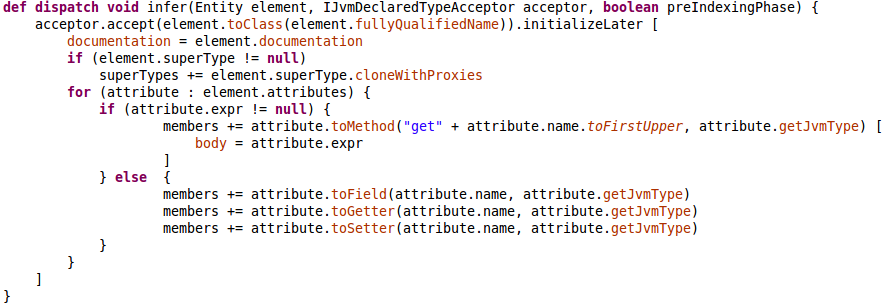
\includegraphics[width=1.1\textwidth]{img/xbase-infer.png}
  \pause
  \begin{itemize}
    \item Entity Attributes $\Rightarrow$ Xbase expressions, Java elements 
   \end{itemize}
  \note{Reuse JVM types by mapping to Java}
\end{frame}    

\note{
\begin{frame}
  \frametitle{\xbaseImpl}
  \begin{itemize}
    \item Entity Attributes $\Rightarrow$ Xbase expressions, Java elements 
   \end{itemize}
   \pause
  \begin{footnotesize}
  % Generator: GNU source-highlight, by Lorenzo Bettini, http://www.gnu.org/software/src-highlite
\begin{tabular}[t]{l}
\noindent
\mbox{}@Inject\ ITypeProvider\ typeProvider \\
\mbox{} \\
\mbox{}\textbf{\textcolor{Plum}{def}}\ JvmTypeReference\ \textcolor{Black}{getJvmType}(Attribute\ attr)\ \{ \\
\mbox{}\ \ \ \ \textbf{\textcolor{Plum}{switch}}\ attr\ \{ \\
\mbox{}\ \ \ \ \ \ \ \ Attribute\ \textbf{\textcolor{Plum}{case}}\ attr.type\ !=\ \textbf{\textcolor{Plum}{null}}\ :\ attr.type \\
\mbox{}\ \ \ \ \ \ \ \ Attribute\ \textbf{\textcolor{Plum}{case}}\ attr.expr\ !=\ \textbf{\textcolor{Plum}{null}}\ :\  \\
\mbox{}\ \ \ \ \ \ \ \ \ \ \ \ \ \ \ \ \ \ typeProvider.\textcolor{Black}{getType}(attr.\textcolor{Black}{getExpr}()) \\
\mbox{}\ \ \ \ \ \ \ \ \textbf{\textcolor{Plum}{default}}:\ \textbf{\textcolor{Plum}{null}} \\
\mbox{}\ \ \ \ \} \\
\mbox{}\}
\end{tabular}

  \end{footnotesize}
\end{frame}
}


\section{Xsemantics}
\label{sec:xsemantics}

Xsemantics~\cite{lbts} (the successor of Xtypes~\cite{Bet11}) is a DSL (written
in Xtext) for writing type systems, reduction rules, interpreters (and in
general relation rules) for languages implemented in Xtext.
A system definition in Xsemantics is a set of judgment rules which have a
conclusion and a set of premises; these rules can act on any Java object,
though, typically, they will act on EObjects which are elements of the metamodel
of the language implemented in Xtext.  Indeed, Xsemantics relies on Xbase to
provide a rich syntax for defining rules (and premises of rule), thus giving
full access to Java types.

Xsemantics is thought to be used by people who are at least a little familiar
with formal type systems and operational semantics: it aims at providing
a syntax which is close to the way deduction rules are written in a formal
setting~\cite{hindley:1997a,Pierce02}.
Actually, Xsemantics rules are written in the other direction with respect
to standard deduction rules: the conclusion come before the premises; this is just
to make IDE tooling work better, and to give a more "programming" style to rules.

Starting from the definitions of these rules, Xsemantics generates Java code
that can be used in your language implemented in Xtext for scoping and
validation (it also generates a validator in Java).  Xsemantics aims at
providing a rich syntax for defining any kind of rules: relations among elements
(e.g., \emph{subtyping}), \emph{static semantics} (i.e., type systems) and
\emph{dynamic semantics} (i.e., reduction rules that can be used for
interpreting a program).  In this paper, we will use it for writing the rules of
the type system of the case study we are considering
(Section~\ref{sec:casestudy}).

\subsection{Type System Specification}

The first thing to do in a system defined in Xsemantics, after giving it a name,
is to declare the \emph{judgments} of your system; a judgment consists of

\begin{itemize}
\item 
a name, which has to be unique in the system;
\item 
a \textit{judgment symbol} that can be chosen from some predefined symbols;
\item 
the \textit{parameters} of the judgment; parameters of a judgments are separated by
	a \textit{relation symbol} that can be chosen from some predefined symbols;
\end{itemize}

\noindent
The parameters can be

\begin{itemize}
\item 
input parameters, in that case they are declared as Java parameters;
\item 
output parameters, in that case you use the keyword
\verb|output| followed by the Java
type of the output parameter.
\end{itemize}

\begin{lstlisting}[language=xsemantics,float,label=lst:xsem-judgments,caption=Judgment
definitions in Xsemantics]
system org.typesys.xsem.guidsl.xsemantics.TypeSystem

import org.typesys.xsem.guidsl.xsemGuiDsl.*

judgments {
	type ||- Typable typable : output Type
	// whether {@code right} is assignable to {@code left}
	isAssignable |- Type left <~ Type right
	// computes the most general type between {@code first} and {@code second}
	mostGeneral |- Type first ~~  Type second |> output Type
}
\end{lstlisting}

\noindent
The judgment definitions for our case study are shown in
Listing~\ref{lst:xsem-judgments}.

Once the judgments of the system are declared, we can start declaring the
rules.  Each rule consists of

\begin{itemize}
\item
a name, which has to be unique in the system;
\item
a \textit{rule conclusion};
\item
the \textit{premises} of the rule;
\end{itemize}

\noindent
The rule conclusion consists of

\begin{itemize}
\item
the name of the \textit{environment} of a rule;
\item
a \textit{judgment symbol};
\item
the \textit{parameters} of the rules, which are separated by
a \textit{relation symbol} that can be chosen from some predefined symbols;
\end{itemize}

The things that make a rule belong to a specific judgment are the judgment
symbol and the relation symbols (which separate the parameters); moreover the
types of the parameters of a rule must be (Java) subtypes of the corresponding types
of the judgment (or exactly the same Java types).  Two rules belonging to the
same judgment must differ for at least one input parameter's type.

The premises of a rule which are specified in a \verb|from| block can be any
Xbase expression, or a rule invocation.  If you think of a rule declaration as a
function declaration, then a rule invocation corresponds to function invocation,
thus you must specify the environment to pass to the rule, and the arguments,
both input and output arguments.
The premises of an Xsemantics rule are considered in \emph{logical and} relation
and are verified in the same order they are specified in the block.
If we need premises (block of premises) in \emph{logical or} relation, we can
use the operator \verb|or|, which separates blocks of premises; if (and only if) one
of the premises of the first block fails, the premises of the second block are
inspected, etc.

Also the concept of rule environment is taken from the type theory (usually is
denoted by the $\g$).  It can be used to pass additional argument to rules.
If you want to be sure to pass an empty environment when invoking a rule you can
use the keyword \mykeyb{empty}.
Furthermore, when passing an environment during a rule invocation, one
can specify additional \emph{environment mapping}, using the syntax
\lstinline[breakatwhitespace=false,breaklines=true]!key <- value!, 
where you can use any Xbase expression;
you can also pass an environment with additional
mappings separated by a comma (or even build an environment from scratch
by specifyin all the mappings, still separated by a comma); for instance
\lstinline[breakatwhitespace=false,breaklines=true]!G, x <- 'foo', y <- 10! 
or
\lstinline[breakatwhitespace=false,breaklines=true]!x <- o.eClass, y <- (o.eClass.name == 'foo')!, 
etc.
Note that when you pass an environment to a rule with additional mappings,
you actually pass a brand new environment, thus you will not modify the
current rule environment; if a mapping already exists in the current rule
environment, in the brand new environment (and only there) the existing mapping
will be overwritten.  Thus, the rule environment passed to a rule acts
in a stack manner.

If a rule does not require any premise, we can use a special form of
rules, called indeed \textit{axiom}s, which only have a conclusion, without
premises.
In the premises you can assign values to the output parameters; and when you
invoke another rule, upon return, the output arguments will have the values
assigned in the invoked rule.

\begin{lstlisting}[language=xsemantics,float,label=lst:xsem-firstrules,caption=Some
examples of rules and axioms in Xsemantics.]
axiom BooleanLiteralType
	G |- BooleanLiteral lit : XsemGuiDslFactory::eINSTANCE.createBooleanType

rule AttributeRefType
	G |- AttributeRef attrRef : Type type
from {
	G |- attrRef.attr : type
}

rule LengthOfType
	G |- LenghtOf len : XsemGuiDslFactory::eINSTANCE.createIntType
from {
	G |- len.expr : var StringType stringType
}

rule FieldContentType
	G |- FieldContent fieldContent : Type type
from {
	G |- env(G, 'widgetcontent', Attribute) : type
}
\end{lstlisting}

In Listing~\ref{lst:xsem-firstrules} we present some rules for the judgment
\mytt{type} (see Listing~\ref{lst:xsem-judgments}, recall that in the rules of
these judgments the second parameter is an output parameter).
For typing a literal (in the example a boolean literal) we write an axiom (since
there is no premise) and the result is a \mytt{BooleanType} (created through the
EMF factory for our language).  The rule for typing an \mytt{AttributeRef} can
be read as follows: the type of an \mytt{AttributeRef} is the type resulting
from typing the corresponding referred attribute (the feature \mytt{attr}, refer
to Listing~\ref{lst:grammar-plain}). The type of a \mytt{LenghtOf} expression is
an integer type, provided that the expression argument of \mytt{LenghtOf} has
string type.  Finally, for typing \mykeyb{widgetcontent} we make use of the
rule environment: we access the environment with the predefined function
\mykeyb{env}, by specifying the key and the expected Java type of the
corresponding value.  If no key is found in the environment or the value cannot
be assigned to the specified Java type the premise will fail.  We will show
how such environment is passed in Section~\ref{sec:xsem-validation}.  Thus, this
rule will type \mykeyb{widgetcontent} with the type of the corresponding
attribute. 

In an hypothetic formal type system, we would probably write these typing rules

\begin{center}
\begin{tabular}{c@{\hspace{.5cm}}c@{\hspace{.5cm}}c}
\inferrule
{}
{\g \f \mykeyb{true} : \mykeyb{boolean} }
&
\inferrule
{\g \f \mytt{attr} : \T}
{\g \f \mykeyb{ref} \ \mytt{attr} : \T }
\\
\\
\inferrule
{\g \f \mytt{exp} : \mykeyb{string}}
{\g \f \mykeyb{lengthOf}(\mytt{exp}) : \mykeyb{int} }
&
\inferrule
{\g \f \g(\mykeyb{widgetcontent}) : \T}
{\g \f \mykeyb{widgetcontent} : \T }
\end{tabular}
\end{center}

\noindent
Note how, the rules in Xsemantics (see Listing~\ref{lst:xsem-firstrules}) remind
of the deduction rules typically used in formal type systems.

At runtime, upon rule invocation, the generated Java system will select the most
appropriate rule according to the runtime types of the passed argument (using
the \textit{polymorphic dispatch} mechanism provided by Xtext).

If one of the premises fails, then the whole rule will fail, and in turn all the
stack of rule invocation will fail.  In particular, if the premise is a boolean
expression, it will fail if the expression evaluates to false.  If the premise
is a rule invocation, it will fail if the invoked rule fails.

As another example, we show in Listing~\ref{lst:xsem-attribute} the rule for
\mytt{Attribute}.  Recall (refer to Listing~\ref{lst:grammar-plain}) that an
attribute can have an explicit type and an initialization expression. The rule
says that in case the type is not explicit the resulting type is the type of the
initialization expression; otherwise, the resulting type is the explicit type of
the attribute; however, in the latter case, if the initialization expression is
specified, then we must make sure that the type of the expression is assignable
to the declared type.

\begin{lstlisting}[language=xsemantics,float,label=lst:xsem-attribute,caption=Type
rule for \mytt{Attribute}.] 
rule AttributeType 
	G |- Attribute attr : Type attrType 
from {
	if (attr.type != null) {
		if (attr.expr != null) {
			G |- attr.expr : var Type expType
			G |- attr.type <~ expType
		}
		attrType = attr.type
	} else {
		G |- attr.expr : attrType
	}
}
\end{lstlisting}

Thus, the rule in Listing~\ref{lst:xsem-attribute} relies on rules of the
judgment \mytt{isAssignable} (see Listing~\ref{lst:xsem-judgments}); the rules
of this judgment, which basically implements subtyping, do not have an output
parameter, they accept two types as parameters; the intention of these rules is
that they succeed if the right parameter is assignable to the left parameter.

\begin{lstlisting}[language=xsemantics,float,label=lst:xsem-assignable,caption=Some
rules for the \mytt{isAssignable} judgment.] 
rule IsAssignableBase
	G |- Type left <~ Type right
from {
	left.eClass == right.eClass
}

axiom BooleanAssignableToString
	G |- StringType left <~ BooleanType right

axiom IntAssignableToString
	G |- StringType left <~ NumberType right

axiom IntAssignableToFloat
	G |- FloatType left <~ IntType right
\end{lstlisting}

In Listing~\ref{lst:xsem-assignable} we present some rules for the
\mytt{isAssignable} judgment.  The first rule is the most general case, and says
that types of the same kind are assignable to each other (in this context
``kind'' corresponds to EClass); moreover, we have some axioms saying that
booleans and integers are assignable to strings (for instance, like in Java, by
an implicit conversion through \mytt{toString} method).  Finally, an integer can
be assigned to a float.

\begin{lstlisting}[language=xsemantics,float,label=lst:xsem-entitysubtyping,caption=Rule
for \mytt{isAssignable} for entity types.] 
rule EntityTypeAssignable
	G |- EntityType left <~ EntityType right
from {
	left.ref == right.ref
	or
	getAll(right.ref, 
		XsemGuiDslPackage::eINSTANCE.entity_SuperType,
		XsemGuiDslPackage::eINSTANCE.entity_SuperType,
		typeof(Entity)
	).contains(left.ref)
}
\end{lstlisting}

In Listing~\ref{lst:xsem-entitysubtyping} we show a more interesting case for
subtyping: the one between two \mytt{EntityType}.  The idea is that \mytt{right}
can be assigned to \mytt{left} either if they are the same type (entity
subtyping is reflexive) or if \mytt{left} is a ``super entity'' (possibly
indirectly) for \mytt{right} (entity subtyping is transitive).  We could check
the latter condition by following recursively the feature \mytt{superType} of
the right entity; however, in an uncorrect program the entity hierarchy might be
acyclic, and this recursive inspection might lead to an infinite loop.  In a
manual Java implementation we thus would have to keep track of the visited
entities while inspecting the hierarchy (see
Listing~\ref{lst:plain-type-conformance}).  Indeed, the AST for Xtext languages,
due to references might be graphs.  Since when developing Xtext languages we
might face the issue of inspecting a graph avoiding possible loops, e.g., to
compute the ``closure'' of a graph, Xsemantics provides a predefined function
which allows to collect nodes in a graph according to EMF features avoiding
loops.  Such function is

\begin{small}
\begin{verbatim}
getAll(eObject, feature to collect, feature to follow, expected type)
\end{verbatim}
\end{small}

\noindent an invocation of \mytt{getAll} will return a list of ``expected
type'', built by collecting all the elements from ``feature to collect'' of the
specified ``eObject'', and recursively collecting such elements by following the
feature ``feature to collect'', but avoiding possible loops in the EMF graph
representing the AST.
Thus, in the use of Listing~\ref{lst:xsem-entitysubtyping}, it will return all
the superclasses of \mytt{right}.  Similarly, we can get all the attributes of
an entity, including the inherited ones, by simply calling

\begin{lstlisting}[language=xsemantics] 
	getAll(entity, 
		XsemGuiDslPackage::eINSTANCE.entity_Attribute,
		XsemGuiDslPackage::eINSTANCE.entity_SuperType,
		typeof(Attribute))
\end{lstlisting}

\begin{lstlisting}[language=xsemantics,float,label=lst:xsem-mostgeneral,caption=Rule
for \mytt{mostGeneral}.] 
rule MostGeneral
	G |- Type first ~~ Type second |> Type mostGeneral
from {
	{
		G |- first <~ second
		mostGeneral = first
	} or
		mostGeneral = second
}
\end{lstlisting}

The judgment \mytt{mostGeneral} (Listing~\ref{lst:xsem-judgments}) takes two
types as input parameters and returns as output the most general between the
two; this judgment has one simple rule, shown in
Listing~\ref{lst:xsem-mostgeneral}.

\begin{lstlisting}[language=xsemantics,float,label=lst:xsem-binaryexp,caption=Some
rules for binary expressions.] 
rule MinusType
	G |- Minus minus : NumberType type
from {
	// require number types
	G |- minus.left : var NumberType leftType
	G |- minus.right : var NumberType rightType
	// get the most general
	G |- leftType ~~ rightType |> type
}

rule PlusType
	G |- Plus plus : Type type
from {
	// deal with any type
	G |- plus.left : var Type leftType
	G |- plus.right : var Type rightType
	// get the most general (which can also be string)
	G |- leftType ~~ rightType |> type
}
\end{lstlisting}

The judgment \mytt{mostGeneral} is useful for typing some binary expressions,
for instance, \mytt{Minus} and \mytt{Plus}, shown in
Listing~\ref{lst:xsem-binaryexp}.  The typing rule for \mytt{Minus} requires
that the two subexpressions have a numeric type (recall that since we specify a
\mytt{NumberType} as the output argument in rule invocation, such invocation
will succeed only if the result is assignable to \mytt{NumberType}); the
resulting type will be the most general type, thus, for instance, if one of the
two subexpressions have type \mytt{FloatType} and the other one \mytt{IntType},
the resulting type will be \mytt{FloatType}.  Recall that we use \mytt{+} not
only as the arithmetic operator, but also for string concatenation; in
particular, if one of the subexpression is a string, the whole expression is
considered as string concatenation.  Thus, the rule for \mytt{Plus} computes the
types of the two subexpressions, and then gets the most general; if one of them
is a string type, the whole expression will have string type (see also subtyping
rules in Listing~\ref{lst:xsem-assignable}).

\subsection{Rules for the Validator}
\label{sec:xsem-validation}

In an Xsemantics we can specify some special rules which do not belong to any
judgment, \mytt{checkrule}, which are used by Xsemantics to generate a Java
validator for the Xtext language.  A \mytt{checkrule} has a name, a single
parameter (which is the EObject which will be checked by the validator) and the
premises (but no rule environment).  The syntax of the premises of a
\mytt{checkrule} is the same of standard rules.
Xsemantics will generate a Java validator with a \checkm{} method for each
\mytt{checkrule}; just like in Java validators for Xtext languages, you can have
many checkrules for the same JavaType (provided the rule name is unique).

\begin{lstlisting}[language=xsemantics,float,label=lst:xsem-validator,caption=Some
checkrules for the Validator.] 
checkrule AttributeTypeChecks for Attribute attribute
from { empty |- attribute : var Type type }

checkrule ValidateMustBeBoolean for Widget widget
from {
	widget.validate == null
	or 
	'widgetcontent' <- widget.attr |- widget.validate : var BooleanType boolType
}

checkrule ValidateTextWidgetAttributeNotBoolean for TextWidget widget
from {
	'widgetcontent' <- widget.attr |- widget.attr : var Type attrType
	!(attrType instanceof BooleanType)
}

checkrule ValidateCheckBoxWidgetAttributeBoolean for CheckBoxWidget widget
from { 'widgetcontent' <- widget.attr |- widget.attr : var BooleanType attrType }
\end{lstlisting}

In Listing~\ref{lst:xsem-validator} we present some checkrules for validating
the elements of our language (see Section~\ref{sec:casestudy}).  The first
checkrule basically says that an Attribute is correct if we can give it a type
(in the empty environment).  The second one accepts a Widget provided that
either its validate part is not specified or it has a boolean type; note that in
this case we pass to the type judgment an explicit environment so that we are
able to type possible occurrences of \mykeyb{widgetcontent}.  These first two
rules also show an important use of environment: since the rule for typing
\mykeyb{widgetcontent} requires that the string `widgetcontent' is bound to an
attribute in the environment, and since when typing an attribute we provide an
empty environment, then a possible occurrence of \mykeyb{widgetcontent} in an
attribute's initialization expression (which is accepted by the grammar) will be
automatically (and correctly) rejected.
The third checkrule requires that the text widget's attribute is not of boolean
type, while the fourth one requires that the checkbox's attribute has a boolean
type (by implicitly trying to assing the result type, in the rule invocation, to
a boolean type).
\subsection{Usage in Xtext}

Xsemantics will generate two Java classes for each xsemantics system:
A Java class with the same name of the system, containing all the
implementations of the system's rules; a derived class from
\mytt{AbstractDeclarativeValidator}, with a \checkm{} for each checkrule (see
Section~\ref{sec:xsem-validation}).
The generated classes rely on Google injection, and they delegate some jobs to
other classes that the programmer can inject to customize the behavior of the
generated code.

The generated validator can be used in conjunction with the language existing
Java validator (so that some checks can be implemented manually and the other
ones rely on the code generated by Xsemantics).  The other Java class,
representing the system written in Xsemantics can be used in all the other parts
of the Xtext implementation of the DSL.  A typical use is in the scope provider,
in languages where the scope of elements highly rely on types, for instance.

The generated Java class containing the rules of your system will have
public methods for the judgments of your system.  For instance, if a judgment is
defined as follows


\begin{lstlisting}[language=xsemantics] 
judgments {
	myjudgment |- MyClass1 arg1 : MyClass2 arg2 : output MyOutputClass
}
\end{lstlisting}

\noindent
the generated Java system will feature three public methods

\begin{lstlisting}[language=Java] 
public Result<MyOutputClass> myjudgment(MyClass1 arg1, MyClass2 arg2)
public Result<MyOutputClass> myjudgment(RuleEnvironment env,
	MyClass1 arg1, MyClass2 arg2)
public Result<MyOutputClass> myjudgment(
	RuleEnvironment env, RuleApplication trace,
	MyClass1 arg1, MyClass2 arg2)
\end{lstlisting}

The class \mytt{Result} is part of Xsemantics runtime, and it is a wrapper for
the actual result value and a possible failure (in the shape of a \failedexc.
The value in the result will be \mytt{null} if the judgment rule failed; in that
case one might want to inspect the \failedexc.
In particular, Xsemantics provides utility methods to get the stack of all the
rule failures (also already formatted as an indented string).
In case the judgment has two output parameters, the class
\mytt{Result2} will be used which acts as a pair.
If the judgment has no output parameter, the type of the result will
be \mytt{Result<Boolean>}.

The first generated method basically only takes the arguments specified in the
judgment.  With the second version, you can also pass an environment
(generated Java code can transparently deal with null environments).
The third one is useful for testing/debugging purposes: if you pass
an instance of \ruleapptrace{} if the
method terminates with success you can then inspect the trace of all the rules
invoked together with the values used in the rules.  If the judgment fails,
you will see also the rules that failed in the rule application trace.
Xsemantics provides utility methods to get a string representation of a trace
indented, with the following idea

\begin{footnotesize}
\begin{verbatim}
final result provided by rule MyRule
 rule 1 used by MyRule to get to the result
  rule 2 used by rule 1
   rule 3 used by rule 2
   ...
 rule 1a used by MyRule to get to the result
  rule 2a used by rule 1a
  ...
\end{verbatim}
\end{footnotesize}


\section{XTS}
\label{sec:xts}

\subsection{Introduction}

XTS was originally developed as a framework with a Java API to declaratively
specify type system rules. Later, a DSL was put on top of the framework which
simply generates the Java code that had to be written before.
If no suitable declarative abstraction is available, either in the framework or
in the DSL, procedural Java code can still be added manually.

XTS features the \ic{ITypesystem} interface. It has various methods for
calculating the type of model elements, and for comparing types for
compatibility and subtyping relationships. To benefit from the framework, it is
recommended to use the declarative APIs from in the \ic{DefaultTypesystem}
implementation.

\subsection{Hooking up the type checker}

To enable type checks, the type system framework  has to be hooked up with the
validation  framework provided by Xtext. Here is the validator code:

\begin{lstlisting}[language=Java] 
@Inject private ITypesystem ts;

@Check(CheckType.NORMAL)
public void validateTypes( EObject m ) {
    ts.checkTypesystemConstraints( m, this );
}    
\end{lstlisting}

The type system can be used in any other place in an Xtext DSL implementation.
For example it has been used as part of scope implementations, in which case the
type system may be reused by injecting it into the scope provider as a field.

\subsection{Setting up}

We start with the header of the type system file.

\begin{lstlisting}[language=xts] 
typesystem org.typesys.xts.guidsl.typesys.GuiDlsTypesystem 
    ecore file 
    "platform:/resource/org.typesys.xts.guidsl/src-gen/org/typesys/xts/guidsl/GuiDsl.ecore"
    language package org.typesys.xts.guidsl.guiDsl.GuiDslPackage 
\end{lstlisting}

The header specifies the fully qualified class name of the type system
implementation class generated from this specification file. We also have to
provide the platform URI for the Ecore file that contains the metaclasses for
which we want to specify the type system rules (the one generated from the Xtext
grammar). Finally, we have to provide the the fully qualified name of the
package class generated from that Ecore file.

\subsection{The type of types}

Type system specifications  are structured into sections. They have no meaning
beyond structuring the overall file. Inside sections we can define \ic{typeof}
clauses. A \ic{typeof} clause defines how the type for a given metaclass is
calculated, and can optionally specify constraints on the types of properties of
these metaclasses.

In the following piece of code we specify  that the type
of the \ic{Type} metaclass and all its subclasses (hence the \ic{+}) is a clone of itself.
In other words, types are their own types.

\begin{lstlisting}[language=xts] 
section "Types"
    typeof Type+ -> clone
    subtype IntType base FloatType
\end{lstlisting}

We also specify the subtyping relationship between \ic{FloatType} and \ic{IntType}. This
means that, wherever a \ic{FloatType} is expected, an \ic{IntType} can also be
used as well.  But not the other way around. In other words, \ic{IntType} is more
specialized.

\subsection{Literals}

The type of string literals and Boolean literals is always the same, so it can
be fixed to a specific type.
However, for number literals it is more complicated:
whether it is an integer or float type depends on the value and this cannot be
expressed declaratively in the DSL. So we declare the type for
\ic{NumberLiteral} to be calculated with Java code.

\begin{lstlisting}[language=xts] 
section "Literals"
      typeof StringLiteral -> StringType
      typeof BooleanLiteral -> BooleanType
      typeof NumberLiteral -> javacode
\end{lstlisting}
 
This specification leads to the generation of an abstract method into the
generated type system class, which we have to override in the manually written
subclass. The corresponding method looks as follows:
 
\begin{lstlisting}[language=Java] 
public EObject type( NumberLiteral s, TypeCalculationTrace trace ) {
    if ( s.getValue().equals(s.getValue().intValue())) {
        return create(cl.getIntType());
    }
    return create(cl.getFloatType());
} 
\end{lstlisting}



\subsection{Expressions}

Before we define the type system rules for the various expressions,  we first
define two characteristics. A \emph{characteristic} is essentially a set of
types. Instead of listing the set of types over and over again, we can use the
characteristic the shortcut.

\begin{lstlisting}[language=xts] 
characteristic COMPARABLE {
    IntType, FloatType, BooleanType, StringType
}  
  
characteristic NUMERIC {
    IntType, FloatType
} 
\end{lstlisting}

Then we define the type for the abstract \ic{Expression} class: it 
has no type, since it is itself abstract, and all it subclasses have different
types. However, it makes sense to declare this fact explicitly, because the type
system DSL editor can then check that all subclasses of \ic{Expression} are actually
covered by type system rules.

\begin{lstlisting}[language=xts]
typeof Expression -> abstract
\end{lstlisting}

We can now take a look at some of the more interesting cases. For comparisons,
the type will be \ic{BooleanType} and the \ic{left} and \ic{right} arguments
have to be \ic{Comparable} (see above). In addition, they also have to be compatible.
For instance, while boolean and string types are both comparable, they cannot be
compared \emph{to each other}. This is why we need this explicit compatibility check:

\begin{lstlisting}[language=xts]
 typeof Comparison -> BooleanType {
     ensureType left :<=: char(COMPARABLE)
     ensureType right :<=: char(COMPARABLE)
     ensureCompatibility left :<=>: right
 } 
\end{lstlisting}


The symbol \verb|:<=:| is called \emph{ordered} compatibility. It
means that the type on the left must be the same or a subtype of the type
specified on the right. The symbol \verb|:<=>:| represents \emph{unordered}
compatibility: the left must be the same or a subtype of the right, or vice
versa.

\begin{lstlisting}[language=xts,float,label=lst:xts-binaryexpressions,caption=Some
rules for expressions.] 
typeof Equality -> BooleanType {
    ensureType left :<=: char(COMPARABLE), BooleanType
    ensureType right :<=: char(COMPARABLE), BooleanType
    ensureCompatibility left :<=>: right
}

typeof AndOrExpression -> BooleanType {
    ensureType left :<=: BooleanType
    ensureType right :<=: BooleanType 
}   

typeof Plus -> common left right {
    ensureType left :<=: StringType, char(NUMERIC)
    ensureType right :<=: StringType, char(NUMERIC)
    ensureCompatibility left :<=>: right
} 

typeof Minus -> common left right {
    ensureType left :<=: char(NUMERIC)
    ensureType right :<=: char(NUMERIC)
    ensureCompatibility left :<=>: right
} 

typeof MultiOrDiv -> common left right { 
    ensureType left :<=: char(NUMERIC)
    ensureType right :<=: char(NUMERIC)
} 

typeof BooleanNegation -> BooleanType {
    ensureType expression :<=: BooleanType
}
\end{lstlisting}

The remainder of specifications for the binary expressions is essentially more
of the same (Listing~\ref{lst:xts-binaryexpressions}).
The only thing worth mentioning is the \ic{common} keyword. Using \ic{common} in the
type for a meta class means that the type is going to be the common supertype of the two
arguments. This only works, if the two types are either the same or part of a
subtype relationship (such as \ic{FloatType} and \ic{IntType}).

Let us now look at some more special cases: the type of the attribute reference
is the type of the referenced attribute. In other words, we have to follow the 
\ic{attr} reference to find out the type:

\begin{lstlisting}[language=xts]
typeof AttributeRef -> feature attr
\end{lstlisting}

The type of the widgets (they are not expressions, but as we will see below, it
is useful if they have a type) should also be relatively straightforward. This
is also where  the type system rules for our test case are finally implemented
(Listing~\ref{lst:xts-widgets}).

\begin{lstlisting}[language=xts,float,label=lst:xts-widgets,caption=Rules
for widgets.] 
// 1) the expression after "validate" must be boolean
typeof Widget -> abstract

// 2) text widgets may only refer to non-boolean attributes 
typeof TextWidget -> feature attr {
    ensureType length :<=: IntType
    ensureType attr :<=: StringType, IntType, FloatType
    ensureType validate :<=: BooleanType
}  

// 3) checkbox widgets may only refer to boolean attributes
typeof CheckBoxWidget -> feature attr {
    ensureType attr :<=: BooleanType
    ensureType validate :<=: BooleanType
}
\end{lstlisting}


We can now calculate the type of the \ic{FieldContent} expression, which has to have
the same type as  the attribute to which the parent widget points. Since we
have defined the type of the widget to be the type of the reference attribute,
we can now use the following type specification for \ic{FieldContent}:

\begin{lstlisting}[language=xts]
typeof FieldContent -> ancestor Widget
\end{lstlisting}

The type of \ic{NewExpr} is the type of the \ic{new}'ed entity:

\begin{lstlisting}[language=xts]
    typeof NewExpr -> feature entity
\end{lstlisting}

 Finally, the type of an \ic{Entity} also has to be calculated with Java code, because
 it has to be an \ic{EntityType} that references the corresponding entity:

\begin{lstlisting}[language=Java]
    protected EObject type(Entity element, TypeCalculationTrace trace) {
        EntityType et = (EntityType)create(cl.getEntityType());
        et.setRef(element);
        return et;
    }
\end{lstlisting}

There is one more interesting open issue. We have to implement the subtyping
relationship between entities. This is not so simple, because we compare
\ic{EntityType}s, and the subtyping depends on whether their corresponding
referenced entities are subtypes of each other. So instead of declaring a
subtype relationship in the DSL, we can implement a type comparison function in
Java. The method \emph{internalCompareTypesOrdered()} checks the entity subtype
relation with cycle detection as seen in the plain Xtext case in listing
\ref{lst:plain-type-conformance}, operation \emph{internalIsAssignable()}.


\begin{lstlisting}[language=Java]
protected boolean compareTypes( EntityType t1, EntityType t2, CheckKind k, TypeCalculationTrace trace ) {
    if ( k == CheckKind.same ) return t1.getRef() == t2.getRef();
    if ( k == CheckKind.ordered ) return internalCompareTypesOrdered(
        t1.getRef(), t2.getRef(), Sets.<Entity>newHashSet());
    return false; 
}
\end{lstlisting}


  


\section{Evaluation}
\label{sec:evaluation}

\todo{there should be some substructure to this section.}

\todo{We should explictly refer back to the functions of type system frameworks
F1 to F5 introduced in the intro.}


The choice of which type system framework to use to implement the type system
for a DSL in Xtext mainly depends on the context of the DSL itself.  In this
section we summarize our experiences, and evaluate the features of the
mechanisms and frameworks described in this paper.

The ``plain Xtext'' strategy (Section~\ref{sec:plain-xtext}) is always feasible,
and, by relying on the powerful features of Xtend, it is even easier to deal
with complex model visits.  However, if the DSL has to rely on an involved type
system, implementing such functionalities in plain Java/Xtend might still be a
big effort.  The complete control on all the parts of the implemented type
system comes at the cost of having to deal with all the internal details,
without relying on any abstraction.  For instance, as shown in
Listings~\ref{lst:plain-type-provider1} and~\ref{lst:plain-type-conformance},
we must avoid possible loops in type computations, and this spreads the actual type system rules in many parts of the
program.

If the DSL has to be tightly integrated with Java, there is basically one single
sensible choice: rely on Xbase.  By ``integration with Java'' we do not only
mean that the DSL must simply be translated into Java (this single requirement does not
prevent from using the other frameworks).  Instead we mean that the DSL must
reuse Java types not only in declarations but also in the actual operation code
(for instance, it must create objects in a Java-like style and invoke methods on
such instances).

With Xbase the DSL ``inherits'' a rich Java-like syntax for expressions (with
functional closures and a type inference mechanism that saves from writing all
types explicitly in declarations) and the complete Java type system; in
particular, the Xbase expression parts of the DSL will be dealt with directly by Xbase itself, relieving the programmer from the big burden of having to reimplement typical type checks.
Notably, Xtend is based on Xbase.
It is also possible to customize
several aspects of Xbase expressions, starting from the syntactic shape of the
expressions (though it might not be possible to change radically such syntax
without experiencing grammar ambiguities) up to the typing and semantics of such
expressions.  The latter scenario, though, might require some deeper knowledge
of Xbase internals (for which, in most cases, the code of Xbase is the only
documentation).  For instance, in Xsemantics itself, Xbase is used for the
syntax of the premises of rules; however, single boolean Xbase expression
statements in the premises of an Xsemantics rule have a different semantics: if
the expression does not evaluate to true the whole rule must fail, while in
Xbase a boolean expression used as a statement is not considered valid (it
represents a statement with no side effect).  To deal with that, in Xsemantics,
a custom validator is implemented to ``intercept'' the checks in the Xbase
validator in order not to issue an error in these situations.
Similarly, a custom Xbase compiler is implemented in Xsemantics in order to wrap
the generated Java code for boolean expressions with appropriate Java code to
deal with possible failures of such expressions.

Thus, the more the DSL is similar to Java, the easier it will be to reuse Xbase
(the Domainmodel example which comes with Xtext is a demonstration).  Otherwise,
things might get more complicated, though it is still possible to customize the
typing and semantics of Xbase expressions.

Xsemantics can be a useful framework for implementing a language which has been
formalized using standard meta-theory mechanisms: define the type system of the
language, its semantics, and then prove that the language is sound by showing
that the semantics is consistent with the type system.
Xsemantics aims at providing a rich syntax for defining any kind of rules:
relations among elements (e.g., \emph{subtyping}), \emph{static semantics}
(i.e., type systems) and \emph{dynamic semantics} (i.e., reduction rules that
can be used for interpreting a program); in particular, this syntax is close to
the way deduction rules are written in a formal
setting~\cite{hindley:1997a,Pierce02} (see Table~\ref{lst:xsem-firstrules}). 
Thus, it is easier to implement the formal definition of type system and operational semantics in Xsemantics, since
the gap between formal systems syntax and the actual implementation is reduced.
Moreover, when implementing type systems in Xsemantics, the details of the
original formal type system are not lost and spread through several lines of
Java (or Xtend) code, and the programmer is relieved from many implementation
details, thanks to the declarative style of Xsemantics rule syntax. For
instance, Xsemantics was used to implement the type system of
\emph{Featherweight Java}~\cite{IgarashiPierceWadler:TOPLAS-2001} (a minimal Java core, used to
prove properties of Java-like languages) which was previously implemented
manually in Xtext~\cite{Bet10}, and to implement type inference with unification
for computing the most general type for a simple \emph{lambda calculus} (see the
examples in~\cite{lbts}).  Furthermore, it is being employed to re-engineer the
implementation of other languages implemented in Xtext, which have a solid
theoretical foundation (\cite{CompDelta,TraitRecordJ-SCP}).

XTS offers its specific syntax for the most common tasks when defining type
constraints. These include specifying that the type of an element is itself,
subtype relationships and compatibility constraints, grouping several elements
(\emph{characteristic}) to save constraint code, and access to EMF features of
model elements which allows to specify that a model element has the type of one
of its features.  Since XTS only targets type systems, the specification of a
type system in XTS is more compact (and less verbose) than Xsemantics (where
judgments for typing and subtyping have to defined explicitly).
XTS has been used in several real-world Xtext DSLs and has
proven to be useful and stable. While a few additional features would be worth
adding to the DSL (e.g. instantiating structured types such as the
\ic{EntityType}), the fact that a few types have to be calculated in Java is not
a big problem in practice.

An important feature that we believe type system frameworks should provide is
the ability to keep a trace of the computation that brings to the derivation of
a type (or of its failure).  This is crucial both for debugging and for testing
the type system.  Both Xsemantics and XTS provide mechanisms for accessing such
traces; instead, when using the direct approach or Xbase, keeping the traces of
type computations must be implemented manually.  In particular, when using
Xbase, this might not be possible since it would require modification of
internal code.  In such cases, debugging the type system might be much harder.

Both Xsemantics and XTS allow to provide custom Java code for specific type
computations, by relying on the \emph{Generation Gap}~\cite{Vlissides:1996:GGS}
pattern: there will be a class that encapsulates generated code and another
class that encapsulates modifications.  In Xsemantics the need of providing
custom Java code is rare since it relies on Xbase for rule implementation, thus
it already has a rich syntax; in XTS more involved type computations (like
entity subtyping) can be delegated to Java code, especially when the access to
EMF features is not directly sufficient to derive a type (or a subtyping
relation).

Finally, Xsemantics and XTS, starting from the specification of the type system
rules in their DSLs, generate automatically an Xtext validator that can already
be used (possibly together with a manually implemented validator); the generated
validator reuses the Java code generated for the type system to check that the
program is correct with respect to types, and to generate errors with
detailed information about typing rules which failed.
This reduces the need of writing additional code: in the plain Xtext
implementation, after writing the code for the type system itself, the validator
still needs to be manually implemented (together with the error information
generation concerning type errors).  Furthermore, having the validator
automatically generated, guarantees consistency between the errors generated and
the type rules, while with the manual approach, one needs to somehow duplicate
efforts.

Summarizing, both Xsemantics and XTS provide all the functionalities that we
outlined in the Introduction, thus they complement Xtext for the implementation
of DSLs which require an involved type system.  In particular, the Java code
generated by these frameworks seamlessly integrate in the validation mechanisms
of Xtext. 


\section{Conclusion and Related Work}
\label{sec:conclusion}

\newcommand{\xtypes}{XTypeS}
\newcommand{\xtext}{Xtext}

A typical way of declaring constraints in metamodels is to use OCL (Object
Constraint Language) \cite{WarmerKleppe99,OCLOMG}.  OCL is an expression
language, while our \xtypes{} is based on type system rules; furthermore, while
OCL is suitable for specifying constraints, it might be hard to use to perform
type inference.

There are other tools for implementing DSLs and their text editors with IDE
functionalities (we also refer to \cite{PP08} for a comparison). Tools like IMP
(The IDE Meta-Tooling Platform) \cite{imp09} and DLTK (Dynamic Languages
Toolkit) \cite{DLTK} only deal with IDE functionalities. TCS (Textual Concrete
Syntax) \cite{tcs} is similar to \xtext, but with the latter it is easier to
describe the abstract and concrete syntax at once, and it is completely open to
customization of every part of the generated IDE (besides, TCS seems to be no
longer under active development). EMFText~\cite{emftext09}, instead of deriving
a metamodel from the grammar, does the opposite, i.e., the language to be
implemented must be defined in an abstract way using an EMF metamodel. Since
also EMFText relies on EMF we believe that \xtypes{} could also be used with
this tool, though we still have not investigated this issue.
Spoofax~\cite{Spoofax2010}, another language workbench which targets Eclipse,
fosters agile language design and development (e.g., changes to the language can
be dynamically loaded into the environment); it does not require Java code for
the analysis of a program (and other IDE related mechanisms) since it relies on
Stratego~\cite{Stratego2008} for rule-based specifications.  With this respect,
\xtypes{} tries to fill the gap concerning the typing of programs, which in
\xtext{} which still requires Java programming, with a type system DSL.

EriLex~\cite{EriLex} is a software tool for generating support code for embedded
domain specific languages and it supports specifying syntax, type rules, and
dynamic semantics of such languages but it does not generate any artifact for
IDE functionalities. MPS (Meta Programming System) \cite{MPS} is another tool
for developing a DSL, and it also provides IDE functionalities, but it does not
target Eclipse and its well-known functionalities.

There are older works that aim at providing complete frameworks for language
implementation (both compilation and editing environment), such as
\emph{Synthesizer}~\cite{Synthesizer} and \emph{Centaur}~\cite{Centaur} (the
former relying on its own specification language and the latter relying on Lisp,
Prolog and other formalisms \cite{Metal,PPML,Typol}). \xtext{} shares with
these tools the philosophy that the editing part is crucial for the programming
(in particular the immediate feedback about problems in the program being
editing~\cite{Synthesizer}) and thus a framework for implementing languages
should address also this functionality.  \xtext, and then \xtypes, aim at
providing these functionalities on top of the widely used Eclipse platform and
by relying on EMF which is a very useful framework for modeling and manipulation
of models (in this case the AST of the programs).

Although \xtypes{} was designed and developed to be used in a language
implemented in \xtext, rules written in \xtypes{} do not refer to the syntax of
the language elements, but only to the structure of the model representing the
AST.  Differently from other approaches, such as, e.g.,
\cite{Centaur,MPS,ASFSDF,Ruler,PLTRedex,EriLex,Neverlang2010}, which require the
programmer to use the framework also for defining the syntax of the language, a
type system written in \xtypes{} only needs an EMF metamodel, i.e., the
\emph{ecore} file (in our context, it is the one generated by \xtext). Thus, the
Java code generated by \xtypes{} might also be used to validate any EMF model,
independently from \xtext{} itself.  Indeed, it might be used with any other
frameworks that represent a program in the shape of an EMF model (though in that
case, Java code generation might have to be adapted).

Neverlang \cite{Neverlang2010} is based on the fact that programming language
features can be easily plugged and unplugged. Similarly, \cite{JastAdd} supports
modular specifications of extensible compiler tools and languages.
Spoofax~\cite{Spoofax2010} provides support for language extensions and
embeddings. \xtext{} provides mechanisms for reusing and composing grammars (we
refer to \xtext{} documentation~\cite{xtext}), but at the moment these
mechanisms may require some manual programming w.r.t.\ the automatic
mechanisms of the above mentioned works. However, from the type system point of
view, since \xtypes{} is only connected to the EMF metamodel (and not to the
grammar), we think that it can be used for modular implementation of type system
related functionalities and in particular for implementing \emph{pluggable type
systems}~\cite{Brac04a}.

\xtypes{} does not aim at providing mechanisms for formal proofs for the
language and the type system; for instance, it does not produce, like other
frameworks do (see, e.g., \cite{Ott}), versions of the type system for proof
assistants like Coq~\cite{Coq}, HOL~\cite{HOL} or Isabelle~\cite{Isabelle}.
Although this issue still needs further investigation, we think that
specifications of rules in \xtypes{} might be good candidates for such generated
definitions for proof assistants.

Finally, we just mention here other tools and frameworks for implementation of
DSLs that are different from \xtext{} and \xtypes{} basically for the main goal
and programming context, such as, e.g., \cite{JST98,MetaBorg06,MontiCore10}
which are based on language specification preprocessors,
\cite{XMF08,LanguageBoxes09} which target host language extensions and internal
DSLs, \cite{ASFSDF,Ruler,PLTRedex} which do not target IDE functionalities. We
would also like to stress that, since \xtypes{} is implemented in \xtext{}
itself, it also provides a full feature Eclipse-based editor for writing the
type system with all the standard IDE functionalities, which is something that
the mentioned related works do not provide.



\bibliographystyle{abbrv} 
\bibliography{lit,lore}
\end{document}
